\section{Infrastructure}



\kimi{3} combines three system challenges rarely encountered in a single model: hybrid KDA attention, 3T-class sparse multimodal training and inference, and million-token agentic workloads. 
Our infrastructure is co-designed with these challenges across the model lifecycle. 
At the architecture level, high-performance KDA kernels and Context Parallelism make the recurrent formulation efficient within and across devices, in both training and inference.
During pretraining, balanced expert execution, reduced memory footprint, and communication-overlapped scheduling sustain high utilization at scale.
During 1M-token agentic RL, hierarchical state management and resumable sandbox execution preserve long trajectories across iterations. 
Finally, state-aware KDA prefix caching, specialized inference kernels, and cache- and budget-aware scheduling translate these efficiencies into predictable production serving.


\subsection{Algorithm-System Co-Design for KDA}
\label{sec:kda-codesign}

KDA replaces the growing key--value cache of softmax attention with a fixed-size recurrent state $\mathbf{S}\in\mathbb{R}^{d_k\times d_v}$ (\S\ref{sec:kda}), whose serial update poses challenges in parallel execution, in exchange for a fixed-size state that is cheap to transfer and reuse.
The designs below address the first property and exploit the second at two levels of execution, with fused kernels within a device and KDA Context Parallelism across devices.

\subsubsection{KDA Kernels across Regimes}
The serial dependence of the KDA state is at odds with the GPU's preference for wide, uniform parallelism, and it manifests as a different bottleneck in each execution regime.
We design a dedicated kernel for each regime.

\paragraph{Chunkwise kernel for training and prefill}
The chunkwise form of KDA is parallel within each chunk but serial across chunks, since the recurrent state must propagate from chunk to chunk.
Executed naively, these two phases alternate, leaving the SMs idle during the serial propagation.
We therefore develop FlashKDA~\citep{flashkda2026}, a CUTLASS-based chunkwise kernel that overlaps intra-chunk computation with cross-chunk state propagation.
The kernel decomposes the work into token-parallel stages and a head-parallel recurrence, each scheduled and tuned independently, and substantially outperforms the Triton reference implementation.
FlashKDA serves both training and inference prefill and is auto-dispatched as a backend of flash-linear-attention~\citep{yang2024fla}.

\paragraph{Intra-device context parallelism for long-context prefill}
Tensor parallelism partitions heads across devices but never shortens the recurrence, so under pure TP deployment, prefilling an ultra-long sequence leaves most SMs idle when each rank holds only a few heads.
The key observation is that the state transition of each segment can be evaluated independently of the incoming state and composed exactly afterward.
An automatic SM-level context-parallel (CP) planner~\cite{yywang2025deltanetcp,yang2024fla} therefore partitions the sequence across the SMs of a single rank, evaluates the segment transitions in parallel, and merges them to recover each segment's exact initial state.
In contrast to the cross-device KCP of \S\ref{sec:kda-cp}, this parallelism is entirely intra-device and incurs no cross-device communication.

KDA decoding presents challenges distinct from those encountered during training and prefill. We discuss these challenges in detail in \S\ref{sec:kda-decoding}.


\subsubsection{KDA Context Parallelism}
\label{sec:kda-cp}

The communication overhead of context parallelism differs fundamentally between softmax and linear attention.
Softmax attention requires ranks to exchange key--value blocks whose size grows with the sequence length~\citep{liu2023ring}.
Linear attention instead carries the preceding context in a fixed-size recurrent state $\mathbf{S}\in\mathbb{R}^{d_k\times d_v}$.
Prior context-parallel methods exploit the additive recurrence of vanilla linear attention by computing, on each rank, the state that the local tokens generate from $\mathbf{S}=\mathbf{0}$ and summing these local states over the preceding ranks to recover the incoming state~\citep{sun2024lasp,sun2025lasp2}.

This direct summation, however, is insufficient for KDA.
Recall from Eq.~\ref{eq:recurrent_KDA} that KDA updates its state as $\mathbf{S}_t=\mathbf{M}_t\mathbf{S}_{t-1}+\beta_t\bm{k}_t\bm{v}_t^{\top}$, where $\mathbf{M}_t:=\left(\mathbf{I}-\beta_t\bm{k}_t\bm{k}_t^{\top}\right)\operatorname{Diag}(\bm{\alpha}_t)$.
KDA's delta rule applies the token-dependent matrix $\mathbf{M}_t$ to the incoming state before adding the current write.
Consequently, the effect of a local sequence segment depends on the state entering that segment and cannot be determined from the state computed with $\mathbf{S}=\mathbf{0}$ alone.

To preserve this dependence, we introduce KDA Context Parallelism (KCP), which decomposes the effect of each segment into two locally computable quantities, a cumulative transition acting on the incoming state and a state generated locally from zero.
Following the chunkwise notation of \S\ref{sec:kda}, we write $\mathbf{S}_{[i]}^{t}$ for the recurrent state within the segment of rank $i$ after $t$ local tokens, so that $\mathbf{S}_{[i]}^{T_i}$ denotes the state leaving rank $i$ and entering rank $i+1$.
We write $\widetilde{\mathbf{S}}_{[i]}^{t}$ for the state of the same recurrence started instead from $\mathbf{S}=\mathbf{0}$.
For an arbitrary state entering the $(i+1)$-th of $P$ context-parallel ranks, the state after $t$ local tokens is
\begin{equation}
    \begin{aligned}
        \mathbf{M}_{[i+1]}^{t \leftarrow 1}
        := \prod_{r \leftarrow 1}^{t}\mathbf{M}_r \in \mathbb{R}^{d_k\times d_k},
        \qquad   \mathbf{S}_{[i+1]}^{t}
         & =\widetilde{\mathbf{S}}_{[i+1]}^{t} + \mathbf{M}_{[i+1]}^{t \leftarrow 1}\mathbf{S}_{[i]}^{T_i}                                                                                                                                    \\
         & = \widetilde{\mathbf{S}}_{[i+1]}^{t} + \mathbf{M}_{[i+1]}^{t \leftarrow 1}\sum_{j=1}^{i}\Big(\prod_{l \leftarrow j+1}^{i}\mathbf{M}_{[l]}^{T_l \leftarrow 1}\Big)\widetilde{\mathbf{S}}_{[j]}^{T_j}\in \mathbb{R}^{d_k\times d_v}.
    \end{aligned}
    \label{eq:kcp-compose}
\end{equation}
\begin{center}
    \begin{adjustbox}{width=\linewidth}
        \definecolor{kcpfigink}{HTML}{1C1C1E}
\definecolor{kcpfiggray}{HTML}{6E6E73}
\definecolor{midnightblue}{HTML}{005C7F}
\definecolor{brickred}{HTML}{B92622}
\definecolor{kvcolor}{RGB}{241,140,74}
\definecolor{kcpgrayd}{HTML}{8A9199}

\tikzset{
        kcpcell/.style={draw=kcpfigink, line width=0.3pt, inner sep=0pt, outer sep=0pt},
        grid4/.style={kcpcell, minimum width=32pt, minimum height=32pt,
                        path picture={
                                        \foreach \r/\a/\b/\c/\d in {0/20/60/10/40,1/70/30/50/20,2/40/80/20/60,3/10/50/30/70} {
                                                        \fill[#1!\a] ([shift={(0,24-8*\r)}]path picture bounding box.south west) rectangle ([shift={(8,32-8*\r)}]path picture bounding box.south west);
                                                        \fill[#1!\b] ([shift={(8,24-8*\r)}]path picture bounding box.south west) rectangle ([shift={(16,32-8*\r)}]path picture bounding box.south west);
                                                        \fill[#1!\c] ([shift={(16,24-8*\r)}]path picture bounding box.south west) rectangle ([shift={(24,32-8*\r)}]path picture bounding box.south west);
                                                        \fill[#1!\d] ([shift={(24,24-8*\r)}]path picture bounding box.south west) rectangle ([shift={(32,32-8*\r)}]path picture bounding box.south west);
                                                }
                                }},
        grid42/.style={kcpcell, minimum width=16pt, minimum height=32pt,
                        path picture={
                                        \foreach \r/\a/\b in {0/20/60,1/70/30,2/40/80,3/10/50} {
                                                        \fill[#1!\a] ([shift={(0,24-8*\r)}]path picture bounding box.south west) rectangle ([shift={(8,32-8*\r)}]path picture bounding box.south west);
                                                        \fill[#1!\b] ([shift={(8,24-8*\r)}]path picture bounding box.south west) rectangle ([shift={(16,32-8*\r)}]path picture bounding box.south west);
                                                }
                                }},
        griddiag/.style={kcpcell, minimum width=32pt, minimum height=32pt,
                        path picture={
                                        \foreach \i/\s in {0/50,1/80,2/30,3/60} {
                                                        \fill[#1!\s] ([shift={(8*\i,24-8*\i)}]path picture bounding box.south west) rectangle ([shift={(8*\i+8,32-8*\i)}]path picture bounding box.south west);
                                                }
                                }},
        gridcol/.style={kcpcell, minimum width=8pt, minimum height=32pt,
                        path picture={
                                        \foreach \r/\s in {0/30,1/50,2/70,3/90} {
                                                        \fill[#1!\s] ([shift={(0,24-8*\r)}]path picture bounding box.south west) rectangle ([shift={(8,32-8*\r)}]path picture bounding box.south west);
                                                }
                                }},
        gridrow/.style={kcpcell, minimum width=32pt, minimum height=8pt,
                        path picture={
                                        \foreach \c/\s in {0/30,1/50,2/70,3/90} {
                                                        \fill[#1!\s] ([shift={(8*\c,0)}]path picture bounding box.south west) rectangle ([shift={(8*\c+8,8)}]path picture bounding box.south west);
                                                }
                                }},
        gridrowv/.style={kcpcell, minimum width=16pt, minimum height=8pt,
                        path picture={
                                        \foreach \c/\s in {0/50,1/90} {
                                                        \fill[#1!\s] ([shift={(8*\c,0)}]path picture bounding box.south west) rectangle ([shift={(8*\c+8,8)}]path picture bounding box.south west);
                                                }
                                }},
        grid42s/.style={kcpcell, minimum width=12pt, minimum height=24pt,
                        path picture={
                                        \foreach \r/\a/\b in {0/20/60,1/70/30,2/40/80,3/10/50} {
                                                        \fill[#1!\a] ([shift={(0,18-6*\r)}]path picture bounding box.south west) rectangle ([shift={(6,24-6*\r)}]path picture bounding box.south west);
                                                        \fill[#1!\b] ([shift={(6,18-6*\r)}]path picture bounding box.south west) rectangle ([shift={(12,24-6*\r)}]path picture bounding box.south west);
                                                }
                                }},
        grid4s/.style={kcpcell, minimum width=24pt, minimum height=24pt,
                        path picture={
                                        \foreach \r/\a/\b/\c/\d in {0/20/60/10/40,1/70/30/50/20,2/40/80/20/60,3/10/50/30/70} {
                                                        \fill[#1!\a] ([shift={(0,18-6*\r)}]path picture bounding box.south west) rectangle ([shift={(6,24-6*\r)}]path picture bounding box.south west);
                                                        \fill[#1!\b] ([shift={(6,18-6*\r)}]path picture bounding box.south west) rectangle ([shift={(12,24-6*\r)}]path picture bounding box.south west);
                                                        \fill[#1!\c] ([shift={(12,18-6*\r)}]path picture bounding box.south west) rectangle ([shift={(18,24-6*\r)}]path picture bounding box.south west);
                                                        \fill[#1!\d] ([shift={(18,18-6*\r)}]path picture bounding box.south west) rectangle ([shift={(24,24-6*\r)}]path picture bounding box.south west);
                                                }
                                }},
        griddiags/.style={kcpcell, minimum width=24pt, minimum height=24pt,
                        path picture={
                                        \foreach \i/\s in {0/50,1/80,2/30,3/60} {
                                                        \fill[#1!\s] ([shift={(6*\i,18-6*\i)}]path picture bounding box.south west) rectangle ([shift={(6*\i+6,24-6*\i)}]path picture bounding box.south west);
                                                }
                                }},
        gridcols/.style={kcpcell, minimum width=6pt, minimum height=24pt,
                        path picture={
                                        \foreach \r/\s in {0/30,1/50,2/70,3/90} {
                                                        \fill[#1!\s] ([shift={(0,18-6*\r)}]path picture bounding box.south west) rectangle ([shift={(6,24-6*\r)}]path picture bounding box.south west);
                                                }
                                }},
        gridrows/.style={kcpcell, minimum width=24pt, minimum height=6pt,
                        path picture={
                                        \foreach \c/\s in {0/30,1/50,2/70,3/90} {
                                                        \fill[#1!\s] ([shift={(6*\c,0)}]path picture bounding box.south west) rectangle ([shift={(6*\c+6,6)}]path picture bounding box.south west);
                                                }
                                }},
}

\begin{tikzpicture}[
                x=1pt,
                y=1pt,
                outer sep=0pt,
                op/.style={font=\footnotesize, text=kcpfigink, inner sep=1pt},
                note/.style={font=\scriptsize, text=kcpfiggray, inner sep=1pt},
        ]
        \path[use as bounding box] (-10,52) rectangle (406,108);

        \node[grid4=brickred] (Mt) at (18,88) {};
        \node[op, right=3pt of Mt] (eq1) {$=$};
        \node[op, right=1pt of eq1] (prod) {$\prod_r$};
        \node[op, right=0pt of prod] (blp) {$\Biggl($};
        \node[op, right=0pt of blp] (lp) {$\Bigl($};
        \node[griddiags=black, right=1pt of lp] (I) {};
        \node[op, right=0pt of I] (minus) {$-$};
        \node[gridcols=midnightblue, right=1pt of minus] (k) {};
        \node[op, right=0pt of k] (times) {$\times$};
        \node[gridrows=midnightblue, anchor=west] at ([shift={(3pt,-3pt)}]k.north east) (kT) {};
        \node[op, right=28pt of k] (rp) {$\Bigr)$};
        \node[griddiag=brickred, right=0pt of rp] (alpha) {};
        \node[op, right=2pt of alpha] (brp) {$\Biggr)$};

        \node[grid42=kvcolor, right=18pt of brp] (s3) {};
        \node[op, right=4pt of s3] (eq3) {$=$};
        \node[grid42=midnightblue, right=4pt of eq3] (t3) {};
        \node[op, right=4pt of t3] (p3) {$+$};
        \node[grid4=brickred, right=4pt of p3] (m3) {};
        \node[op, right=3pt of m3, yshift=-1pt] (sumj) {$\sum\nolimits_j$};
        \node[grid4=brickred,opacity=0.4] at ($(sumj.east)+(23,3)$) (m2b) {};
        \node[grid4=brickred, right=4pt of sumj] (m3b) {};
        \node[grid42=midnightblue, right=7pt of m3b] (s1in3) {};

        \coordinate (sepmid) at ($(alpha.east)!0.5!(s3.west)$);
        \draw[draw=kcpfiggray, line width=0.4pt, dash pattern=on 3pt off 3pt]
        ([shift={(0,3)}]sepmid |- Mt.north) -- ([shift={(0,-3)}]sepmid |- Mt.south);

        \node[note, below=12pt of Mt, anchor=base] {$\mathbf{M}_{[i+1]}^{t \leftarrow 1}$};
        \node[note, anchor=base] at ($(I |- alpha.south)!0.5!(kT |- alpha.south)+(0,-12)$) {$\mathbf{I}-\beta_r\bm{k}_r\bm{k}_r^{\top}$};
        \node[note, below=12pt of alpha, anchor=base] {$\operatorname{Diag}(\bm{\alpha}_r)$};
        \node[note, below=12pt of s3, anchor=base] {$\mathbf{S}_{[i+1]}^{t}$};
        \node[note, below=12pt of t3, anchor=base] {$\widetilde{\mathbf{S}}_{[i+1]}^{t}$};
        \node[note, below=12pt of m3, anchor=base] {$\mathbf{M}_{[i+1]}^{t \leftarrow 1}$};
        \node[note, below=12pt of m3b, anchor=base] {$\prod_l\mathbf{M}_{[l]}^{T_l \leftarrow 1}$};
        \node[note, below=12pt of s1in3, anchor=base] {$\widetilde{\mathbf{S}}_{[j]}^{T_j}$};
\end{tikzpicture}

    \end{adjustbox}
\end{center}
where $\mathbf{M}_{[i+1]}^{t \leftarrow 1}$ denotes the cumulative transition of the first $t$ local tokens.
The first term contains the state generated by the local tokens, whereas the second term propagates the context from preceding ranks through the local KDA updates.
At $t=T_{i+1}$, both quantities $\mathbf{M}_{[i+1]}^{T_{i+1} \leftarrow 1}$ and $\widetilde{\mathbf{S}}_{[i+1]}^{T_{i+1}}$ can be computed using only the local tokens, before $\mathbf{S}_{[i]}^{T_i}$ is available, and are the fragments each rank exchanges with the others.

The summation in Eq.~\ref{eq:kcp-compose} shows that every state is composed purely from locally computed fragments.
These rank-level updates compose associatively, so the incoming state of each rank can be recovered by a prefix scan~\citep{martin-2018-parallelizing}.
Each rank first computes $\mathbf{M}_{[i]}^{T_i \leftarrow 1}$ and $\widetilde{\mathbf{S}}_{[i]}^{T_i}$ locally, then exchanges both tensors with one \texttt{all-gather}~\citep{yang2024fla}.\footnote{
    The construction builds on DeltaNet context parallelism~\citep{yywang2025deltanetcp}.
    The KDA implementation is available in \href{https://github.com/fla-org/flash-linear-attention/pull/691}{FLA PR~\#691}.
}
After the \texttt{all-gather}, rank $i+1$ reconstructs $\mathbf{S}_{[i]}^{T_i}$ by processing preceding fragments of the same document in order, starting from $\mathbf{S}=\mathbf{0}$ and applying $\mathbf{S}\leftarrow\mathbf{M}_{[j]}^{T_j \leftarrow 1}\mathbf{S}+\widetilde{\mathbf{S}}_{[j]}^{T_j}$ at each fragment.
Therefore, KCP requires only a fixed-size \texttt{all-gather} for recurrent-state synchronization and achieves linear compute scaling.



\subsection{Infra for 3T-class Pre-Training}
\label{sec:infra-training}


\kimi{3} pre-training combines Pipeline Parallelism (PP) with virtual stages (VP)~\citep{huang2019gpipe, narayanan2021efficient}, Expert Parallelism (EP)~\citep{lepikhin2020gshard}, ZeRO-1 Data Parallelism~\citep{rajbhandari2020zero}, Pipeline ZeRO-2 gradient sharding~\citep{glm5team2026glm5vibecodingagentic}, and Context Parallelism (CP, \S\ref{sec:kda-cp})~\citep{jacobs2023deepspeedulyssesoptimizationsenabling}.
The MoE layers employ shared experts replicated across EP ranks, and the all-to-all communication for expert dispatch and combine is overlapped with computation to hide its latency.

Natively multimodal pre-training at the 3T-class poses three critical problems: (i) token loads are imbalanced across EP ranks; (ii) activations, gradients, and optimizer states exceed the memory budget; and (iii) the vision encoder's highly variable computation is exposed on the critical path.
The following subsections address these problems in turn: perfectly balanced expert-parallel MoE training (\S\ref{sec:moe_moonep}), memory-efficient training (\S\ref{sec:memory-efficient-training}), and multimodal encoder optimization (\S\ref{sec:multimodal-encoder-optimization}).
Fig.~\ref{fig:k3pp} illustrates the resulting execution schedule.

\begin{figure}
    \centering
    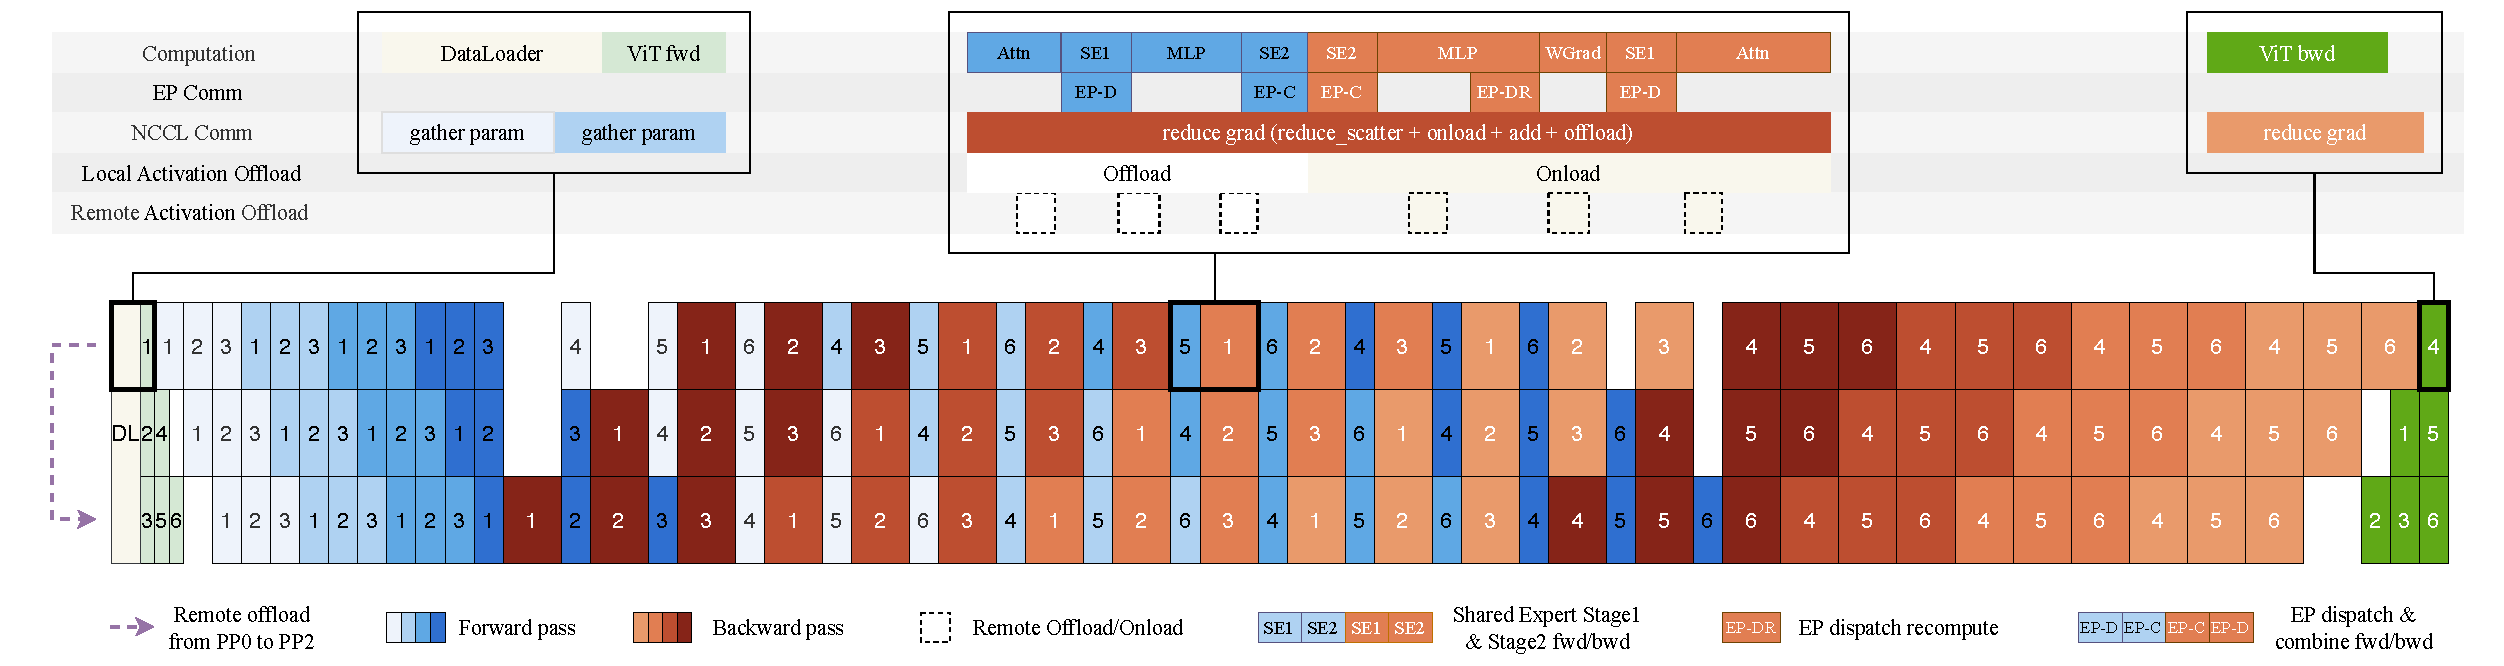
\includegraphics[width=1\linewidth]{figures/k3pp.pdf}
    \caption{Computation, communication and offloading overlapped in different PP phases.}
    \label{fig:k3pp}
\end{figure}


\subsubsection{Perfectly Balanced Expert-Parallel MoE Training}
\label{sec:moe_moonep}
In conventional EP schemes, token loads are imbalanced across ranks.
The resulting computational imbalance degrades training throughput, and the dynamically varying shapes of routed-expert activations cause substantial memory fragmentation.
We therefore propose MoonEP\footnote{\url{https://github.com/MoonshotAI/MoonEP}}, an EP scheme that achieves perfect load balance with dynamic redundant experts.
MoonEP preserves the overall computation flow of conventional schemes such as DeepEP~\citep{deepep2025} and additionally introduces online planning and migration of redundant experts.
In the forward pass, we plan the redundant experts from the router outputs of the current micro-batch and layer and prefetch them before the routed-expert computation.
In the backward pass, we stage their gradients in a local reduce buffer and, once the computation completes, reduce them back to the gradient buffers of their home ranks.

\paragraph{Perfect balance with bounded redundant experts}
MoonEP requires every rank to receive exactly $S \times K$ tokens, where $S$ is the sequence length and $K$ is the number of experts selected per token, so that all ranks perform identical amounts of computation.
The key question is how many redundant experts suffice to guarantee such a balance.
Let $E$ be the number of experts and $R$ the EP size.
We prove that a balanced plan always exists with at most $E/R$ redundant experts per rank and that this bound is essentially tight (\S~\ref{app:moonep-proof}).
Reserving $E/R$ redundant-expert slots per rank therefore guarantees that planning always admits a feasible solution, so training is never interrupted.
In contrast, prior work such as ECHO~\citep{yan2026scalabletrainingmixtureofexpertsmodels} and UltraEP~\citep{wei2026ultraepunleashmoetraining} presets the number of redundant experts or imposes a per-rank token cap.
Training is then forced to stop whenever no feasible plan exists within the cap, and the cap itself requires manual tuning while still leaving residual imbalance.

\paragraph{Online planning}
Computing the exact optimum at every training step is prohibitively expensive.
We therefore compute exact solutions offline with integer linear programming (ILP) for representative cases as references and design a GPU planning kernel that is near-optimal, incurs negligible overhead, and always respects the $E/R$ upper bound.

\paragraph{Zero-copy communication}
Perfect balance also simplifies the communication path.
We implement a fused permute/unpermute operator in which the planning kernel precomputes the destination of every token, so tokens are sent directly to their expert-grouped positions on remote ranks, and views of the communication buffer are returned directly to the computation, eliminating intermediate copies.
Under worst-case imbalance, supporting the same copy-free data path in DeepEP requires a communication buffer of size $S \times K \times R$, whereas MoonEP requires only a fixed $S \times K$ buffer owing to the perfect balance.

\paragraph{Sync-free execution with static shapes}
In conventional MoE implementations, the per-expert token counts vary across steps and layers, and the host must synchronize with the device at every layer to obtain the actual computation shapes before launching the expert computation, stalling the pipeline between layers.
With perfect balance, every rank receives exactly $S \times K$ tokens and the computation shapes of all layers are statically known. This eliminates the per-layer MoE host synchronization and alleviates the host-side kernel-launch overhead.


\paragraph{Expert-GEMM scheduling and overlap}
Even with the aggregate load perfectly balanced across ranks, the per-expert token counts within each rank remain skewed, and a fixed-order, workload-oblivious schedule turns this skew into an imbalanced makespan across SM workers.
We therefore schedule the routed-expert GEMM with a workload-aware scheduler that adapts its parameters to the current token distribution before launch and keeps them fixed during execution.
A lightweight heuristic selects these parameters using an analytical cost model of hardware metrics, with key coefficients calibrated through offline autotuning.
For the shared experts, we dispatch their GEMMs to a separate stream so that they overlap with other kernels.

\subsubsection{Memory-Efficient Training}
\label{sec:memory-efficient-training}

\paragraph{Unified activation manager}
We design a unified storage abstraction for activations, in which every tensor saved for the backward pass is associated with a pluggable storage backend.
Recomputation, quantization, and offload/remote-offload are merely storage policies under this abstraction and can be freely composed at tensor granularity; policies are declared via lightweight annotations on tensors, fully decoupled from the model code.
Recomputation is performed at function granularity, which supports cross-layer recomputation.
In our implementation, all GPU memory is allocated on the main compute stream and managed within a single memory pool, avoiding multi-stream fragmentation and host-bound overhead; activations are prefetched back at layer granularity and overlapped with computation, introducing negligible extra overhead.
In \kimi{3}, most activations use block-wise FP8 quantization~\citep{kimiteam2025kimik2openagentic, deepseekaiv3} combined with offload/remote-offload, and element-wise operators are configured with recomputation.

\paragraph{Memory-efficient MoE}
In the native MoE implementation, the gradient computation of permuted probs depends on the forward output \texttt{output}.
Inspired by SonicMoE~\citep{guo2025sonicmoeacceleratingmoeio}, we rewrite this gradient through a mathematical transformation into a form that depends only on the intermediate activation \texttt{act\_output} and the upstream gradient \texttt{doutput}, eliminating the backward dependency on \texttt{output} at the cost of an additional lightweight element-wise computation.
Furthermore, in the forward pass of the group GEMM, we save only the input of the dispatch operation; during the backward pass, the input of the group GEMM is recovered by recomputing dispatch.
As shown in Fig.~\ref{fig:k3pp}, the communication introduced by this recomputation can be overlapped with part of the group-GEMM backward computation, eliminating this portion of activation storage at a negligible cost.

\paragraph{Memory-efficient Attention residual}
For the attention residual, we design a companion optimization based on Block AttnRes.
The block representation is generated once at the boundary layer and shared by all subsequent layers, residing directly on the GPU.
The AttnRes computation is entirely wrapped with checkpointing, so the activation saved for the backward pass at each layer is identical to that of the standard residual architecture.
For pipeline parallelism, we adopt cache-based pipeline communication~\citep{kimiteam2026attnres}, in which only newly generated blocks are incrementally transferred between stages and released as soon as the micro-batch finishes, reaching the theoretical lower bound on memory footprint.

\paragraph{Balancing activations across PP ranks}
Under interleaved 1F1B pipeline parallelism, activations are unevenly distributed across PP ranks due to pipeline warmup, and the number of resident activations decreases as the PP rank increases.
To avoid out-of-memory (OOM) errors, we remotely offload activations to the memory of other PP ranks using the Mooncake Transfer Engine~\citep{qin2024mooncake}, achieving balanced activation memory across PP ranks.

\paragraph{Pipeline ZeRO-2 gradient sharding and offloading}
\label{para:pipeline-zero2}
Beyond activations, we use Pipeline ZeRO-2 gradient sharding~\citep{glm5team2026glm5vibecodingagentic} to shard gradients across data-parallel (DP) ranks.
Furthermore, we store the sharded gradients in CPU memory to reduce peak GPU memory usage, while keeping the double grad buffer on the GPU.
After gradients are reduced across DP ranks into the double grad buffer, they are accumulated into the CPU shards.

\paragraph{P2P-based Muon orthogonalization}
The distributed optimizer shards parameters evenly across DP ranks, whereas the Newton--Schulz orthogonalization in Muon requires the full parameter matrix, necessitating a communication step to gather complete parameters before each update.
The naive approach performs an all-gather over the entire parameter buffer on every rank~\citep{liu-2025-moonlight}, which incurs a substantial memory footprint on top of making communication the primary bottleneck at scale.
Instead, each rank retrieves only the shards of its locally owned parameters via peer-to-peer (P2P) communication with the corresponding owner ranks, eliminating the full-parameter buffer and reducing both memory usage and communication volume.
Communication and computation are further pipelined at the granularity of model-chunk buffers, hiding the communication overhead.

























\subsubsection{Multimodal Encoder Optimization}
\label{sec:multimodal-encoder-optimization}





\paragraph{Dynamic CP in multimodal encoder}
In long-context multimodal training, large images and long videos substantially increase the computation time of the vision encoder and cause significant load imbalance across devices.
To address this, we extend context parallelism to such large samples.
A single large image is partitioned along the patch dimension across multiple devices, and attention is computed by gathering key--value pairs (gather-KV) across CP ranks.
In addition, we divide each CP group into several sub-CP groups and distribute multiple large images across them in a load-balanced manner, preventing the communication fraction from growing with scale.
This reduces both the encoder latency of large visual samples and the cross-device load imbalance, allowing the remaining encoder computation to be hidden in pipeline bubbles.

\paragraph{Encoder computation in PP bubbles}
In \kimi{2.5}, we introduced the Decoupled Encoder Process (DEP)~\citep{kimik25}, which splits ViT and text training into separate stages and balances vision forward and backward passes across PP stages.
We observe that, under the interleaved 1F1B pipeline schedule, the text forward passes of the first PP micro-batches are all scheduled at the very beginning, while the text backward passes of the last PP micro-batches finish only at the very end.
We therefore further decompose the ViT computation.
The ViT forward passes of the first PP micro-batches are executed synchronously upfront, the remaining forward passes are scheduled into pipeline bubbles, and the backward passes are handled analogously.
As a result, most of the ViT computation is hidden within pipeline bubbles, largely eliminating the effective overhead of the vision encoder.






\subsection{Infra for 1M Agentic RL}

Scaling agentic RL for a model as large as \kimi{3} to million-token contexts under a bounded compute budget makes resource efficiency a first-order goal. This motivates two complementary efforts: 1) efficient training and rollout, including KV-cache management, request scheduling, and training-state placement; 2) high-performance resumable sandboxes for long-horizon interaction.

\subsubsection{Long-context RL infrastructure}
We adopt co-located RL training \cite{kimiteam2025kimik2openagentic} to keep each 1M-context \kimi{3} RL experiment within a few hundred GPUs, and use partial rollouts~\cite{kimik15} to reduce tail latency from ultra-long trajectories. This design achieves good hardware utilization, but introduces a memory usage contention between rollout KV-cache that needs to be persisted for the next iteration, and the memory needed for training. This challenge becomes more severe in long-context RL.

\paragraph{External KV cache pool}
At 1M-context multi-step rollout, a prefix KV-cache miss is extremely expensive. Partial rollout exacerbates this issue at the beginning of each iteration, due to many unfinished long prefill requests from the previous iteration arriving at the same time. Speculative decoding further accelerates request turnover within relatively fixed tool-call intervals, increasing prefix-block churn. These issues can trigger preemption and lower the cache hit rate, which is critical for long-context RL.

We therefore decouple prefix retention from GPU residency with a write-back design.
Active decoding blocks remain in GPU KV cache, while reusable idle prefixes are written back to an \textit{external KV cache pool} in CPU DRAM only when it is evicted from GPU, and is prefetched back before the next reuse.
KDA states are offloaded and prefetched together with the corresponding MLA KV cache blocks, keeping their lifecycles aligned.
Compared with a write-through strategy, this policy incurs CPU DRAM usage and transfer bandwidth only for prefixes that leave the active decode path, avoiding redundant CPU copies of blocks that are still resident and active on GPU.

To provide sufficient DRAM for the external pool, we offload training states (model weights and optimizer states) to NVMe after a training iteration finishes. After a rollout iteration, the pool is released to avoid contention with training workloads.

\paragraph{Rollout auto-throttling scheduler}
In multi-step rollout, contexts grow progressively as the trajectory advances, making fixed concurrency based on the full-trajectory average length both hard to estimate and overly conservative early on.
Conversely, setting concurrency too high creates KV cache pressure in later stages and can trigger preemption.
We therefore design an auto-throttling mechanism at the LLM request scheduling layer, using runtime signals such as active request count, queued request count, and KV cache utilization to dynamically control how many requests are sent to the inference engine.
This keeps early rollout well utilized while reducing concurrency as KV cache pressure rises, avoiding both under-saturation and overload without manual tuning.

\paragraph{Gradient-buffer reuse for non-policy model forwarding}
RL loss computation often requires forward-only non-policy models, such as reference models, whose weights are too large to keep resident on GPU.
We keep these weights in CPU memory and materialize them only when needed, backing their parameter tensors with the policy model's FP32 gradient-buffer storage.
This reuses existing GPU memory without extra allocation or fragmentation, and remains safe because the buffers are overwritten when real gradients are later computed.

With ZeRO-2 gradient sharding and offloading (\S~\ref{para:pipeline-zero2}), each GPU retains gradient buffers for only two VPP chunks in \kimi{3} RL training.
We stream reference weights into these slots chunk by chunk: one slot is used for the current forward computation while the other prefetches the next chunk, hiding copy overhead without increasing GPU memory.

\subsubsection{Sandbox Infrastructure}
\label{sec:sandbox}

We employ multiple sandbox runtimes to support the diverse requirements of \kimi{3} post-training and evaluation, including a traditional container-based runtime, a GPU sandbox runtime, and, most notably, a new microVM-based sandbox runtime called AgentENV.

AgentENV\footnote{AgentENV is open-sourced at \url{https://github.com/kvcache-ai/AgentENV}}, developed in collaboration with our partners, is a sandbox system specifically designed for agentic AI workloads.
It is built around three core design goals:

\begin{itemize}[leftmargin=12pt]

    \item \textbf{High-fidelity isolated sandbox runtime} As agents become more capable and tasks more difficult, they tend to explore more aggressively and may even attempt reward hacking.
          On the one hand, this poses unique security challenges: in our early experiments with traditional container-based sandbox runtimes, we observed several kernel panics and deadlocks caused by unintended agent operations.
          On the other hand, we want to permit as much exploration as possible so as not to constrain agent capability, and complex tasks require a sandbox close to a real-world environment --- for example, agents should be able to mount disks, run containers, or even launch virtual machines at will.
          By running isolated microVMs with Firecracker~\citep{agache2020firecracker}, AgentENV provides a level of isolation and fidelity that container-based runtimes cannot match.

    \item \textbf{Flexible sandbox life-cycles for agentic RL} At the low level, AgentENV supports incremental checkpointing and resuming of sandbox states, where only memory pages dirtied since the last checkpoint are saved during checkpointing, achieving checkpoint and resume latencies as low as 133\,ms and 49\,ms, respectively.
          On top of this, AgentENV provides three high-level operations that help improve agentic RL efficiency.
          \textbf{(a) Pause and Resume}: a paused sandbox consumes no memory or CPU resources; a sandbox can therefore be paused while the agent is waiting for the model's inference result, which can account for as much as 98\% of the sandbox lifetime.
          \textbf{(b) Fork}: fork creates a new sandbox from the exact state of the original one while keeping the original running, which is useful for reward judging without side effects.
          \textbf{(c) Snapshot}: snapshots of a sandbox can be saved at regular intervals for error recovery.

    \item \textbf{High efficiency and high density} In our workloads, tens of thousands of sandboxes, each with a unique set of images, may need to be created within seconds.
          We adopt OverlayBD~\citep{li2020dadi} as the image format, together with a custom ublk driver implementation, storage-layer sharing, and P2P transport, achieving sub-second launch latency at large scale.
          We further reduce memory usage with copy-on-write memory and page-cache optimizations, achieving a memory overcommit ratio of up to 6.5$\times$ in real workloads.

\end{itemize}

Throughout \kimi{3}'s training and evaluation, a total of 51{,}219{,}741 sandboxes across 1{,}505{,}678 images were created.


\subsection{Inference and Online Serving}
\label{sec:inference}

Serving \kimi{3} exposes the same challenges from the production side: the hybrid KDA--MLA architecture maintains two fundamentally different caches that must be managed jointly at million-token contexts, its new modules and highly sparse experts demand kernels tailored to each, and production traffic mixes requests whose per-request cost spans three orders of magnitude.
The designs below address these challenges at three levels.
At the engine level, a KDA-aware prefix cache packs the fixed-size recurrent state into the same paged pool as the MLA KV cache and keeps long prefixes reusable across requests.
At the device level, dedicated kernels for KDA decoding, Block AttnRes, and the sparse latent MoE minimize per-token latency and memory traffic.
At the fleet level, cache-aware affinity scheduling and budget-based admission control translate these efficiencies into predictable serving.

\subsubsection{KDA-Aware Prefix Cache Management}

The hybrid architecture in \kimi{3} complicates prefix caching: the KDA recurrent state and the MLA KV cache differ fundamentally in size and lifetime, yet a cached prefix is reusable only when both can be restored together at the same boundary.
We therefore design a KDA-aware prefix cache that manages the two cache types jointly---from a unified paged layout to fine-grained prefix reuse and consistency under concurrent scheduling---keeping million-token prefixes cheap to retain and reusable across requests.

\paragraph{Unified cache layout for hybrid KDA--MLA attention}
Each \kimi{3} block consists of three KDA layers and one Gated MLA layer, whose caches differ fundamentally.
The MLA KV cache grows with sequence length and is paged per token, whereas the KDA recurrent state is fixed in size with a single copy per request.
Maintaining a separate manager for each would duplicate the allocation, eviction, and transfer logic.
We therefore pack KDA states into the same paged block pool as MLA KV, unifying pages to the same byte size so that both page types share one implementation of allocation, reference counting, and eviction.
Within a page, the states of all heads are stored contiguously head by head, so that each head's byte stream is self-contained and serves as the minimal unit of cross-node transfer.
Under prefill/decode disaggregation, when prefill and decode nodes adopt different TP degrees, re-layout is performed on the transfer path with zero GPU-side reshuffling.
This asymmetry proved useful during development: any type-confused access yields garbage rather than plausible data --- a zero-overhead sanity check on the pooled layout.


\paragraph{KDA prefix cache optimization}





Block-hash-based prefix caching reuses the KV cache at the granularity
of one physical block: only complete blocks are hashed, so only
block-aligned prefixes are reusable.

This coupling breaks down in \kimi{3}. Block-hash matching requires
one block size shared by all layers, and a prefix hit is reusable only
if the KDA state at the hit boundary has been persisted. A KDA layer
maintains a single large recurrent state per sequence rather than
per-token entries, so state snapshots are affordable only at sparse
boundaries; the shared block size is therefore forced to 1024--6144
tokens---and, since hashing is tied to the storage block, the hash
granularity as well, although MLA's per-token entries alone would
tolerate much finer blocks. At such a coarse granularity caching is
nearly useless: requests shorter than one block can never be reused,
and chunked prefill exports no cacheable prefix until it crosses a
full block boundary.


\begin{figure}[!hb]
    \centering
    \begin{tikzpicture}[font=\small]
        \def\hbw{0.92}  % width of one prefix-hash block
        \foreach \i in {0,...,11} {
                \pgfmathsetmacro{\x}{\i*\hbw}
                \ifnum\i<5\relax
                    \fill[blue!20] (\x,0) rectangle (\x+\hbw,0.5);
                \else
                    \fill[black!6] (\x,0) rectangle (\x+\hbw,0.5);
                \fi
            }
        \draw (0,0) rectangle (12*\hbw,0.5);
        \foreach \i in {1,...,11} { \draw (\i*\hbw,0) -- (\i*\hbw,0.5); }
        \draw[decorate,decoration={brace,amplitude=4pt}] (0,0.6) -- (12*\hbw,0.6)
        node[midway,above=4pt,font=\footnotesize]
        {physical cache block (6144 tokens) = 12 prefix-hash blocks};
        \draw[decorate,decoration={brace,amplitude=2.5pt,mirror}] (2*\hbw,-0.08) -- (3*\hbw,-0.08)
        node[midway,below=3pt,font=\footnotesize] {hash block (512 tokens)};
        \node[font=\footnotesize,anchor=west] at (-1.45,0.25) {MLA KV};
        \node[font=\footnotesize,anchor=west] at (-1.45,-0.9) {KDA ckpt};
        \draw[dashed,thick] (5*\hbw,0.5) -- (5*\hbw,-0.9);
        \foreach \k in {1,...,12} { \draw[black!40] (\k*\hbw,-0.9) circle (0.05); }
        \foreach \k in {3} { \fill[black!55] (\k*\hbw,-0.9) circle (0.07); }
        \fill[orange!90!black] (5*\hbw,-0.9) circle (0.10);  % checkpoint hit at B
        \node[font=\footnotesize,anchor=north] at (5*\hbw,-1.0)
        {hit boundary $B=2560$};
        \draw[-{Stealth[length=2.2mm]},thick] (5*\hbw,-1.55) -- (5*\hbw,-1.95);
        \node[font=\footnotesize,anchor=north,align=center] at (6.5*\hbw,-2.0)
        {restore the KDA checkpoint at $B$; copy-on-write the partial MLA block;\\
            resume prefill from token $B$ with zero recompute of $[0,B)$};
    \end{tikzpicture}
    \caption{\textbf{Fine-grained prefix caching within a physical cache block.}
        A 6144-token physical block contains twelve 512-token hash blocks, with cached MLA blocks shown in blue and empty blocks in light gray.
        The markers below show the KDA checkpoint status at each hash boundary.
        An open circle ($\circ$) denotes a boundary without a stored checkpoint, a gray dot (\textcolor{black!55}{$\bullet$}) denotes a persisted KDA checkpoint, and an orange dot (\textcolor{orange!90!black}{$\bullet$}) marks the checkpoint hit at $B=2560$.
        Persisted checkpoints are sparse and typically coincide with conversation-turn boundaries.
        The request reuses the five MLA hash blocks and the KDA checkpoint at $B$, then resumes prefill without recomputing $[0,B)$.}
    \label{fig:kda-prefix-cache}
\end{figure}


We therefore decouple the two granularities. Prefix hashing runs on
fine \emph{hash blocks} (e.g., 512 tokens) inside MLA pages, while the
physical block remains the coarse allocation unit. Alignment runs the
other way for KDA: checkpoints of the recurrent state are saved only
at (a sparse subset of) MLA's hash endpoints---the only positions a
lookup can ever reference.

During prefill, a partially filled MLA page is registered in the
prefix-cache index under the chained hash of its last complete hash
block, where each hash covers all preceding hash blocks so that
matching an endpoint certifies the whole prefix up to it; the
registered endpoint advances as the page fills. Meanwhile, after each
forward pass, the KDA kernel persists the recurrent state at the last
hash-aligned position processed. Checkpoints are large, so
intermediate checkpoints superseded as the request advances are
recycled, while those at conversation-turn boundaries are retained for
cross-request reuse. Cached checkpoints are read-only snapshots: a hit
restores the state by copying it into the request's private running
state before the next forward pass, and new checkpoints are written to
fresh slots, so a checkpoint visible to other requests is never
mutated in place.



Lookup proceeds in two stages (Fig.~\ref{fig:kda-prefix-cache}). The
MLA stage matches whole physical blocks by chained hash and, at the
first missing block, falls back to the hash endpoints inside it, so
partially filled pages remain hittable. The KDA stage then requires a
checkpoint at the candidate boundary in every KDA cache group, each of
which maintains an independent recurrent state. The hit is the longest
boundary satisfying both stages---always a multiple of the hash block,
and never required to be a multiple of the physical block. In
Fig.~\ref{fig:kda-prefix-cache}, a request whose first 2800 tokens
match the cached prefix hits at $B=2560=5\times512$, deep inside a
6144-token physical block, and resumes prefill from token $B$ instead
of recomputing $[0,B)$.


\paragraph{Consistency under concurrent scheduling}
The remaining design points are each dictated by a concrete failure mode of sharing partially filled blocks, in a setting where a hit block is at once a shared cache entry and the growth point of a private request, and where the MLA and KDA cache groups must agree on every hit boundary.
First, all cache groups draw blocks from one shared free list, so allocating a private copy for one group could evict a block that another group has just hit; every hit block is therefore pinned across all groups before anything is allocated.
Second, the copy into the private block executes on the GPU immediately before the forward pass, so a block allocated or registered within the current scheduling step would still hand the previous owner's bytes to a reader; such blocks are excluded from matching until their copies land.
Third, a checkpoint can restore a request only if it exists in every KDA group, so evicting one group's checkpoint atomically invalidates its siblings --- a checkpoint is either hittable in every group or in none.
With these mechanisms, every registered state always corresponds to exactly its declared token prefix, and prefix caching for hybrid KDA--MLA models reaches the same generality as for full-attention models: any shared prefix is reusable at any 512-token boundary, independently of request length, chunking, or scheduling interleaving.



\subsubsection{High-Performance Kernels}
\kimi{3} introduces several new architectural modules: KDA (\S\ref{sec:kda}), Block AttnRes (\S\ref{sec:attnres}), and Stable LatentMoE (\S\ref{sec:stable-latent-moe}). We optimize the kernel implementation for each.

\paragraph{KDA}
\label{sec:kda-decoding}

Compared with KDA prefill (\S\ref{sec:kda-codesign}), KDA decoding presents a distinct set of challenges: the primary bottleneck shifts from exploiting parallelism to efficiently managing the evolving recurrent state, which is updated in place at every decoding step. This in-place update becomes problematic in MTP-based speculative decoding: if verification rejects a subset of the drafted tokens, the state has already advanced beyond the last accepted token and cannot be trivially rolled back. Maintaining a state snapshot for each draft position would enable rollback, but would also multiply state traffic --- a cost that dominates at the large batch sizes typical of online serving.


The state after any accepted draft prefix, however, is fully determined by the projected inputs of the draft tokens, which are far smaller than the state itself.
We therefore cache only these projected inputs, rebuild the states of accepted tokens on-chip, and write back the states of the verified and bonus tokens, a design independently proposed in the concurrent work ReplaySSM~\citep{replayssm2026}.
The replayed tokens, the bonus token, and the next draft window share one recurrent loop inside a single fused kernel covering short convolution, input normalization, gating, the KDA recurrence, and output normalization.
Verification latency grows sub-linearly with the number of tokens verified and remains below that of state-caching baselines.
Because the projection caches never leave the decode stage, prefix caching and prefill--decode disaggregation operate on the same payload as in non-speculative serving.

\paragraph{Block AttnRes}
Block AttnRes~\citep{kimiteam2026attnres} follows a two-phase schedule: a batched inter-block pass reads the cached block representations once per block, after which each layer folds in the intra-block partial sum through an online-softmax merge~\citep{milakov2018online}.
Memory access accounts for a substantial fraction of the cost of these kernels in both prefill and decoding, so our optimizations in both stages focus primarily on memory efficiency.

For prefill, materializing the block representations on every tensor-parallel (TP) rank would incur substantial redundant memory consumption. We therefore adopt sequence parallelism (SP) for activations: the TP all-reduce is decomposed into a reduce-scatter and an all-gather, with the intra-block kernel inserted between the two collectives, operating on the sequence-sharded hidden states so that the block representations of each token are materialized on exactly one rank.
This eliminates the additional memory consumption and reduces the I/O overheads of Block AttnRes during prefill.

For decoding, we launch the inter-block kernel on a side stream so that it overlaps with independent computation on the main stream. The intra-block kernel is instead streamlined through fusion: the merging of the AttnRes output with its partial-sum update, together with the subsequent RMSNorm, is fused into the preceding TP all-reduce, eliminating a dedicated kernel for the intra-block phase.
Together, these optimizations hide the latency of the inter-block pass and reduce the memory traffic of the intra-block phase.


\paragraph{Stable LatentMoE}

Stable LatentMoE increases both the total number of experts and the number of activated experts per token. The resulting growth in both the expert space and the per-token expert count raises scheduling and coordination overheads, making it difficult for conventional MoE kernels to sustain high hardware utilization. These challenges motivate dedicated kernel optimizations for this module.


To mitigate the overhead of the latent GEMMs, we adopt three optimizations. First, we fuse the latent down-projection with the MoE router into a single GEMM. Second, we shard latent weight matrices across ranks and fuse the output all-gather into the GEMM epilogue using multimem store instructions. Finally, we overlap the resulting communication with other operators, such as the shared-expert computation. Together, these optimizations eliminate redundant weight traffic and duplicated computation, while hiding the communication latency behind computation.


For routed experts, at small batch sizes, the group GEMMs reduce to memory-bound streaming of weight matrices --- a regime for which conventional tile-centric kernels are poorly suited due to their compute-oriented design and preprocessing overheads.
We instead build the MoE decoding kernel upon the token-centric design of WarpDecode~\citep{warpdecode2026}, in which each warp is responsible for one output neuron and streams the associated weights directly from memory. To further increase parallelism, we subdivide each warp into finer-grained lane teams, each processing a disjoint subset of experts, followed by a warp-wide reduction of the partial results. In addition, the weight layout is permuted offline at a one-time preprocessing cost, substantially reducing the runtime dequantization overhead.








\subsubsection{Fleet-Level Scheduling}
Beyond a single serving instance, the challenge shifts from per-request efficiency to predictability: a prefix-cache miss costs orders of magnitude more than a hit, and a burst of million-token requests can starve short ones.
We propose two fleet-level scheduling policies to address this: cache-aware affinity scheduling routes each session to the cluster holding its prefix cache while bounding the cost of cluster failures, and budget-based admission control grants each request class its own resource budget so that bursty long-context traffic cannot degrade system-wide SLOs.


\paragraph{Cache-aware affinity scheduling}
At 1M context, a typical coding input carries a prefix of 400K tokens but requires a prefill increment of only 4K tokens, so a prefix-cache hit avoids re-prefilling the entire prefix and is orders of magnitude cheaper than a miss.
We therefore route each request to the cluster that holds its prefix cache, as moving the cache to another cluster would require transferring it over inter-cluster links far slower than the intra-cluster fabric.
This cache-aware affinity, however, binds each session to a single cluster, whose failure would interrupt all sessions bound to it.
Consistent hashing therefore pins each session to two clusters, a primary that serves its traffic and a pre-assigned secondary that takes over when the primary fails.
The secondary holds none of the session's prefix cache and must re-prefill it upon failover.
Since consistent hashing distributes the secondary assignments of different sessions uniformly across the fleet, this re-prefill work is divided among many clusters rather than concentrated on one.
Cache locality is thus preserved in the common case, while the impact of any single cluster failure remains bounded.

\paragraph{Budget-based admission control}
Production traffic mixes short requests under 2K tokens with ultra-long requests up to 1M tokens, so the per-request cost spans roughly three orders of magnitude and the total load imposed by any fixed number of requests is highly unpredictable.
Capacity planning, queueing models, and rate-limiting quotas based on the ``average request'' all break down under this variance.
In a typical failure mode, a burst of long-context requests saturates the available compute, and short requests arriving afterwards cannot be scheduled promptly, degrading time to first token (TTFT) across all traffic.
We therefore adopt budget-based admission control, allocating separate resource budgets to different request classes so that bursty long-context traffic consumes at most its own share of the capacity and cannot degrade system-wide SLOs experienced by other classes.